\documentclass[a4paper]{article}
\usepackage[
				pdftex,
				colorlinks=true,
				bookmarksnumbered=true,
				bookmarksopen=true,
				bookmarksopenlevel=3,
				pdfstartview=FitP,
				urlcolor=blue,
			]{hyperref}
\pdfinfo{
			/Title(Esercitazione di Laboratorio: Circuiti con diodi)
			/Author(Coa Giulio, Licastro Dario, Montano Alessandra)
		}
\usepackage[italian]{babel}
\usepackage{geometry,titling,mdsymbol,stmaryrd,graphicx,subcaption,amsmath}
\graphicspath{{./Image/}}
\renewcommand\maketitlehooka{
								\null
								\mbox{}
								\vfill
							}
\renewcommand\maketitlehookd{
								\vfill
								\null
							}
\title{
		\begin{center}
			Esercitazione di Laboratorio:
		\end{center}
		\newline
		\begin{center}
			Circuiti con diodi
		\end{center}
	}
\author{
			Coa Giulio
			\and
			Licastro Dario
			\and
			Montano Alessandra
		}
\begin{document}
	%-----------------------------------------------------------------------------
	%  TITLE
	%-----------------------------------------------------------------------------
	\begin{titlingpage}
		\maketitle
	\end{titlingpage}
	\newpage
	%-----------------------------------------------------------------------------
	%  PURPOSE OF THE EXPERIENCE
	%-----------------------------------------------------------------------------
	\section{Scopo dell'esperienza}
		Lo scopo di questa esercitazione è stato analizzare vari circuiti contenenti diodi, tramite l’esecuzione di una serie di misure in condizioni statiche al fine di determinare la caratteristica statica $ I_{\mathrm{d}}(V_{\mathrm{d}}) $ dei suddetti diodi, e la successiva visualizzazione del loro comportamento con una tensione d'ingresso di tipo sinusoidale.
	%-----------------------------------------------------------------------------
	%  INSTRUMENTATION USED
	%-----------------------------------------------------------------------------
	\section{Strumentazione utilizzata}
		La strumentazione usata durante l'esercitazione è:
		\begin{center}
			\begin{tabular}{ |c|c|c| }
				\hline
				\multirow{\textbf{Strumento}}	 & \textbf{Marca e Modello} & \textbf{Caratteristiche} \\
				\hline
				\multirow{Multimetro}			 & Agilent 34401A			& \\
				\multirow{Oscilloscopio}		 & Rigol DS1054Z			& 4 canali, \\
												 &							& $ B = 50 \, \mathrm{MHz} $, \\
												 &							& $ f_{\mathrm{c}} = 1 \, \mathrm{G\frac{Sa}{s}} $, \\
												 &							& $ R_{\mathrm{i}} = 1 \, \mathrm{M\Omega} $, \\
												 &							& $ C_{\mathrm{i}} = 13 \, \mathrm{pF} $, \\
												 &							& $ 12 \, \mathrm{Mbps} $ di profondità di memoria \\
				\multirow{Generatore di segnali} & Rigol DG1022				& 2 canali, \\
												 &							& $ f_{\mathrm{uscita}} = 20 \, \mathrm{MHz} $, \\
												 &							& $ Z_{\mathrm{uscita}} = 50 \, \mathrm{\Omega} $ \\
				\multirow{Alimentatore in DC}	 & Rigol DP832				& 2 canali, \\
												 &							& $ f_{\mathrm{uscita}} = 20 \, \mathrm{MHz} $, \\
												 &							& $ Z_{\mathrm{uscita}} = 50 \, \mathrm{\Omega} $ \\
				\multirow{Sonda}				 & Rigol PVP215				& $ B = 35 \, \mathrm{MHz} $, \\
												 &							& $ V_{\mathrm{nominale}} = 300 \, \mathrm{V} $, \\
												 &							& $ L_{\mathrm{cavo}} = 1.2 \, \mathrm{m} $, \\
												 &							& $ R_{\mathrm{s}} = 1 \, \mathrm{M\Omega} $, \\
												 &							& Intervallo di compensazione: $ 10 \div 25 \, \mathrm{pF} $ \\
				\multirow{Cavi coassiali}		 &							& Capacità dell'ordine dei $ 80 \div 100 \, \mathrm{p\frac{F}{m}} $ \\
				\multirow{Connettori}			 &							& \\
				\multirow{Breadboard}			 &							& \\
				\multirow{Resistenza}			 &							& $ R = 9.9 \, \mathrm{k\Omega} $ \\
				\multirow{Diodo Zener}			 & 1N5228					& \\
				\multirow{Diodo}				 & 1N4148					& \\
				\multirow{Condensatori}			 &							& $ C_{1} = 10 \, \mathrm{nF} $, \\
												 &							& $ C_{2} = 100 \, \mathrm{nF} $, \\
												 &							& $ C_{3} = 1 \, \mathrm{\mu F} $ \\
				\hline
			\end{tabular}
		\end{center}
	%-----------------------------------------------------------------------------
	%  THEORETICAL PREMISES
	%-----------------------------------------------------------------------------
	\section{Premesse teoriche}
		\subsection{Incertezza sulla misura dell'oscilloscopio}
			La misura del valore di un segnale tramite l’oscilloscopio (sia esso l'ampiezza, la frequenza, il periodo, etc.) presenta un'incertezza che dipende, principalmente, da due fattori:
			\begin{itemize}
				\item l’incertezza strumentale introdotta dall’oscilloscopio (ricavabile dal manuale).
				\item l’incertezza di lettura dovuta all’errore del posizionamento dei cursori.
			\end{itemize}
			Quest’ultima incertezza deriva dal fatto che il segnale visualizzato non ha uno spessore nullo sullo schermo.
		\subsection{Sonda}
			La sonda è un particolare cavo coassiale che presenta un'estremità capace di effettuare delle misurazioni.
			\newline
			Quando si usano dei classici cavi coassiali BNC-BNC al fine di collegare il circuito, su cui effettuare le misure, all'oscilloscopio, si sta inserendo in parallelo al circuito un condensatore di capacità ($ C_{\mathrm{c}} $) pari a quella del cavo.
			\begin{figure}[h!]
				\centering
				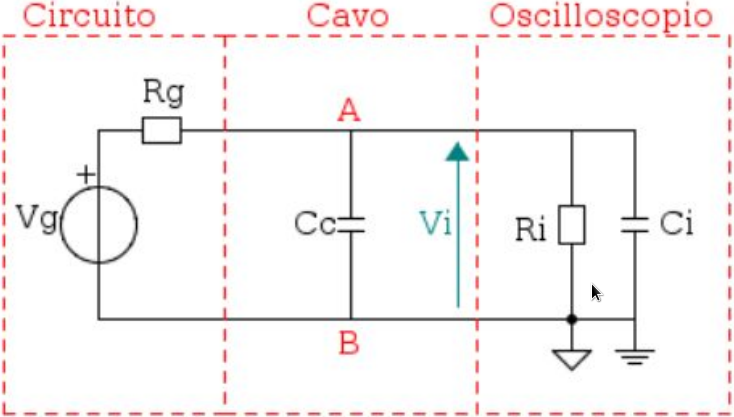
\includegraphics[scale=0.4]{theveninCavoDSO}
				\caption{Circuito analizzato collegato all'oscilloscopio tramite un cavo coassiale BNC-BNC.}
				\label{fig:theveninCavoDSO}
			\end{figure}
			\newpage
			In questo caso, l’oscilloscopio si comporta, in ingresso, come un filtro passa-basso con una frequenza di taglio ($ f = \frac{1}{2\pi R_{i} (C_{s} + C_{i})} $). L'uso di una sonda per misurare delle grandezze in un circuito, si può vedere come l'inserimento di un condensatore in serie al circuito.
			\begin{figure}[h!]
				\centering
				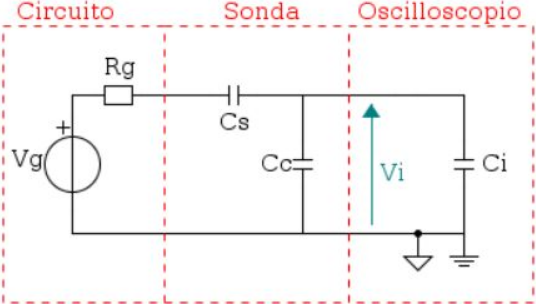
\includegraphics[scale=0.4]{theveninSondaDSOCircuito}
				\caption{Circuito analizzato collegato all'oscilloscopio tramite una sonda.}
				\label{fig:theveninSondaDSOCircuito}
			\end{figure}
			\newline
			L'introduzione di questo condensatore comporta un calo della capacità equivalenti vista all'ingresso del circuito ($ \mathrm{\frac{C_{s} (C_{c} + C_{i})}{C_{s} + C_{c} + C_{i}} \ll C_{c} + C_{i}} $), ovvero una riduzione della frequenza del polo ($ f_{\mathrm{polo}} = \frac{1}{2\pi R_{i} (C_{s} + C_{i})} $); ciò porta ad una perdita d'informazioni in bassa frequenza.
			\newline
			Al fine di evitare tale perdita d'informazioni, si pone, in parallelo al condensatore, una resistenza.
			\begin{figure}[h!]
				\centering
				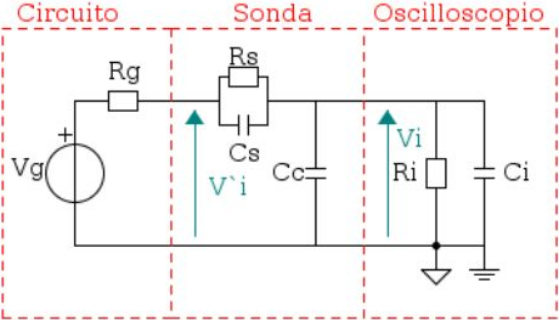
\includegraphics[scale=0.4]{theveninSondaDSOResistenza}
				\caption{Circuito analizzato collegato all'oscilloscopio tramite una sonda.}
				\label{fig:theveninSondaDSOResistenza}
			\end{figure}
			\newline
			Tale resistenza comporta la presenza di uno zero, oltre al polo precedentemente detto.
			\begin{figure}[h!]
				\centering
				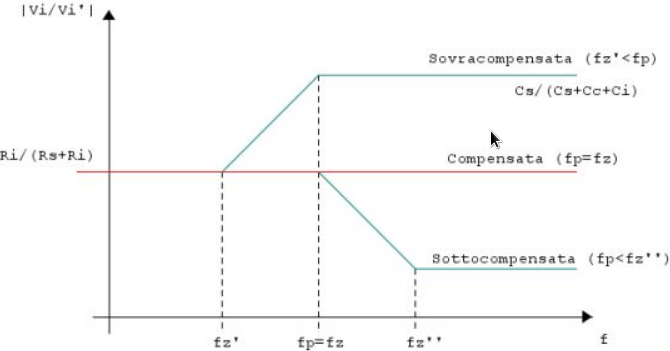
\includegraphics[scale=0.4]{sondaBode}
				\caption{Diagramma di Bode della funzione di trasferimento del circuito.}
				\label{fig:sondaBode}
			\end{figure}
			\newpage
			A seconda dell'elevata o della bassa compensazione della sonda, il segnale sarà distorto verso l'alto o verso il basso.
			\begin{figure}[h!]
				\centering
				\begin{subfigure}{0.4\textwidth}
					\centering
					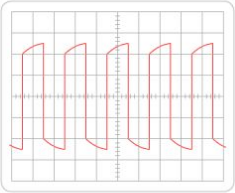
\includegraphics[scale=0.5]{sondaSegnaleSottocompensato}
					\caption{Sonda sottocompensata.}
				\end{subfigure}
				\begin{subfigure}{0.4\textwidth}
					\centering
					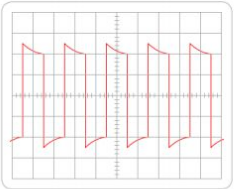
\includegraphics[scale=0.5]{sondaSegnaleSovracompensato}
					\caption{Sonda sovracompensata.}
				\end{subfigure}
				\caption{Visualizzazione del segnale al variare della compensazione della sonda.}
				\label{fig:sondaSegnaleNonCompensato}
			\end{figure}
			\newline
			La sonda risulta compensata quando la frequenza del polo coincide con la frequenza dello zero; ciò avviene quando $ R_{\mathrm{s}} C_{\mathrm{s}} = R_{\mathrm{i}} (C_{\mathrm{c}} + C_{\mathrm{i}})} $. La sonda presenta un opportuno trimmer che influenza il valore di $ R_{\mathrm{s}} $ e permette la compensazione. Al fine di verificare se la sonda è compensata si esegue un confronto con un segnale noto.
			\begin{figure}[h!]
				\centering
				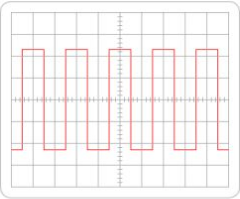
\includegraphics[scale=0.5]{sondaSegnaleCompensato}
				\caption{Sonda compensata.}
				\label{fig:sondaSegnaleCompensato}
			\end{figure}
		\subsection{Diodo}
			Il diodo è un bipolo non lineare il cui comportamento è descritto dalle due seguenti espressioni analitiche equivalenti tra loro
			\newline
			\begin{center}
				$ i_{\mathrm{D}} = I_{\mathrm{S}} \cdot (e^{\mathrm{\frac{v_{\mathrm{D}}}{\eta \cdot V_{\mathrm{T}}}}} - 1) $
			\end{center}
			\newline
			\begin{center}
				$ v_{\mathrm{D}} = \eta \cdot V_{\mathrm{T}} \cdot \ln (\frac{i_{\mathrm{D}}}{I_{\mathrm{S}}} + 1) $
			\end{center}
			dove $ V_{\mathrm{T}} $ è la tensione termica del diodo.
			\begin{figure}[h!]
				\centering
				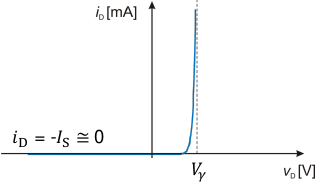
\includegraphics[scale=0.7]{caratteristicaStatica}
				\caption{Caratteristica statica di un diodo.}
				\label{fig:caratteristicaStatica}
			\end{figure}
			\newpage
			Si noti come, al crescere di $ v_{\mathrm{D}} $, la corrente $ i_{\mathrm{D}} $, ovvero la corrente che attaversa il diodo, aumenti (regione di polarizzazione); in particolare, dopo il raggiungimento della tensione di soglia $ V_{\mathrm{\gamma} $, il diodo tende a comportarsi come un generatore ideale indipendente di tensione di valore pari a $ V_{\mathrm{\gamma} $.
			\newline
			Al contrario, quando $ v_{\mathrm{D}} $ è troppo bassa, la corrente $ i_{\mathrm{D}} $ è pari a $ -I_{\mathrm{S}} $, ovvero circa nulla; ciò porta il diodo a comportarsi similmente ad un circuito aperto (regione di polarizzazione inversa). Questa condizione può dare luogo al fenomeno del breakdown, ovvero quando il diodo conduce in direzione opposta; tale fenomeno porta, solitamente, alla rottura del diodo.
			\subsubsection{Diodo di Zener}
				Sono particolari tipi di diodi proggettati appositamente per lavorare anche in polarizzazione inversa; questi diodi non si rompono se si verifica il breakdown, anzi sono caratterizzati da una tensione di soglia negativa, detta, per l'appunto, tensione di breakdown.
				\begin{figure}[h!]
					\centering
					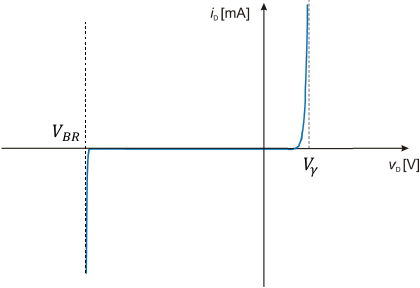
\includegraphics[scale=0.7]{caratteristicaStaticaDiodoZener}
					\caption{Caratteristica statica di un diodo di Zener.}
					\label{fig:caratteristicaStaticaDiodoZener}
				\end{figure}
		\subsection{Raddrizzatore a semplice semionda}
			Circuito fondamentale che, data una tensione in input, caratterizzata da un valor medio non nullo, ne estrae la parte positiva; il segnale in uscita presenta valor medio nullo.
			\newline
			\begin{center}
				$ i_{\mathrm{D}} = I_{\mathrm{S}} \cdot (e^{\mathrm{\frac{v_{\mathrm{D}}}{\eta \cdot V_{\mathrm{T}}}}} - 1) $
			\end{center}
			f(n)=
			\begin{cases}
				n/2, & \mbox{se }n\mbox{ pari} \\ 3n+1, & \mbox{se }n\mbox{ dispari}
			\end{cases} 
			\begin{figure}[h!]
				\centering
				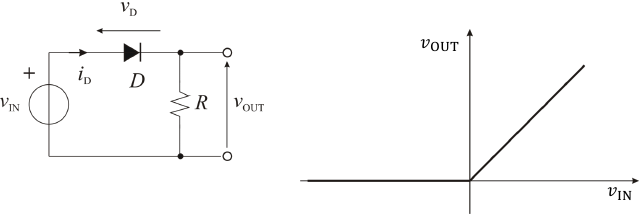
\includegraphics[scale=0.7]{transcaratteristicaStaticaRaddrizzatoreASempliceSemionda}
				\caption{Circuito e transcaratteristica statica di un raddrizzatore a semplice semionda.}
				\label{fig:transcaratteristicaStaticaRaddrizzatoreASempliceSemionda}
			\end{figure}
		\subsection{Protezione ESD}
			Circuito usato come protezione da scariche elettrostatiche, caratterizzato dall'imposizione di una tensione massima e di una tensione minima.
			\newline
			\begin{center}
				$ \Biggl\{ \Biggr\} $
			\end{center}
			\begin{figure}[h!]
				\centering
				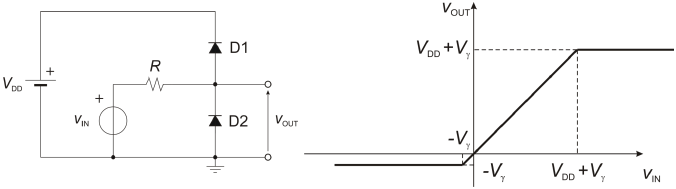
\includegraphics[scale=0.7]{transcaratteristicaStaticaProtezioneESD}
				\caption{Circuito e transcaratteristica statica di una protezione ESD.}
				\label{fig:transcaratteristicaStaticaProtezioneESD}
			\end{figure}
	%-----------------------------------------------------------------------------
	%  LABORATORY EXPERIENCE
	%-----------------------------------------------------------------------------
	\section{Esperienza in laboratorio}
		\subsection{Caratteristiche statiche}
			Abbiamo montanto sulla basetta la resistenza, il diodo D=1N4148 e l'elemento di collegamento.
			Per mezzo del multimetro abbiamo misurato la resistenza e abbiamo verificato la correttezza del valore misurato confrontandolo con il valore della resistenza riportato dal produttore, tenendo conto della sua incertezza.
			Abbiamo connesso la basetta all'alimentatore tramite due cavi a banana, quello rosso a connettere i poli positivi, quello nero usato per la messa a terra, dopodichè abbiamo variato la tensione in ingresso secondo i valori fornitici, ed abbiamo misurato, con il multimetro, i valori di tensione ai capi della resistenza.
			
			In seguito abbiamo connesso, al posto dell'alimentatore, il generatore di segnali alla basetta con un cavo BNC-banana, impostato ampiezza di picco $ V_{\mathrm{p}} = 5 \, \mathrm{V} $ e $ f = 1 \, \mathrm{kHz} $, dando come input il segnale sinusoidale caratterizato da queste due grandezze.
			Abbiammo connesso la sonda ... e osservato i cambiamenti che il diodo ha apportato al segnale.
			
			Abbiamo ripetuto la procedura con il diodo di zener.
		\subsection{Raddrizzatore a semplice semionda}
			Abbiamo costruito i circuito richiesto, aggiungendo il condensatori e sostituendo il diodo zener con il precedente.
			Abbiamo misurato prima le tensioni picco-picco al variare del condensatore, abbiamo potuto apprezzare come la capacità di quest'ultimo influenzi il segnale in uscita rendendolo più o meno (approssimato?).
			In seguito abbiamo ripetuto l'esperienza 
			
		\subsection{Rivelatore di picco}
			.
		\subsection{Circuito per la protezione da scariche elettrostatiche}
			.
	%-----------------------------------------------------------------------------
	%  RESULTS
	%-----------------------------------------------------------------------------
	\section{Risultati}
		\subsection{Caratteristiche statiche}
			\subsubsection{Diodo}
			I risultati ottenuti al variare della tensione in ingresso, fornita con l'alimentatore, sono stati riportati nella seguente tabella.
			%aggiungere una colonna per la caratteristica
			\begin{center}
				\begin{tabular}{ |c|c| }
					\hline
					\multirow{\textbf{Tensione in input [$ \mathrm{V} $]}}	 & \textbf{Tensione in output} \\
					\hline
					\multirow{$ -4 $}										 & $ -0.046 \, \mathrm{mV} $ \\
					\multirow{$ -3.5 $}										 & $ -0.043 \, \mathrm{mV} $ \\
					\multirow{$ -3 $}										 & $ -0.038 \, \mathrm{mV} $ \\
					\multirow{$ -2 $}										 & $ -0.032 \, \mathrm{mV} $ \\
					\multirow{$ -1 $}										 & $ -0.027 \, \mathrm{mV} $ \\
					\multirow{$ 0 $}										 & $ 0.001 \, \mathrm{mV} $ \\
					\multirow{$ 0.2 $}										 & $ 2.067 \, \mathrm{mV} $ \\
					\multirow{$ 0.4 $}										 & $ 45.306 \, \mathrm{mV} $ \\
					\multirow{$ 0.6 $}										 & $ 0.177 \, \mathrm{V} $ \\
					\multirow{$ 0.8 $}										 & $ 0.344 \, \mathrm{V} $ \\
					\multirow{$ 1 $}										 & $ 0.526 \, \mathrm{V} $ \\
					\multirow{$ 1.5 $}										 & $ 0.997 \, \mathrm{V} $ \\
					\multirow{$ 2 $}										 & $ 1.477 \, \mathrm{V} $ \\
					\hline
				\end{tabular}
			\end{center}
			Si può notare che il diodo utilizzato non è adatto alla polarizzazione inversa, infatti per tensioni negative otteniamo valori molto bassi che, però, si mantengono intorno allo $ 0 $. Inoltre abbiamo toccato e superato la tensione di soglia (deve essere minore di $ 0 $ ?).
		
			% RIPORTARE GRAFICO DELLA TANSCARATTERISTICA E DELLA CARATTERISTICA
			
			Dopo aver connesso generatore di segnali, sonda e oscilloscopio (GIULIO NON HO SPEIFICATO COME ABBIAMO CONNESSO LE ROBE PERCHE' E' NELLA PARTE DELLE PREMESSE)abbiamo ottenuto le seguenti immagini, dove il segnale di input è rappresentato dalla linea blu e l'output da quella gialla. 
			%foto 3
			Si può notare come l'input sia un segnale sinusoidale standard, mentre l'output è distorto per effetto del cisrcuito, in particolare la parte negativa del segnale è stata portata a 0 (poichè le tensioni negative ricevute in input dal diodo diventano 0 in output), ed anche la curva sinusoidale risulta un po' schiacciata (perchè?).
			
			In seguito, per misurare l'ampiezza di picco del segnale di output abbiamo posizionato i cursori come in figura ottenendo Vu(t) = 4.440V %ho letto bene?
			%transcaratteristica statica Vu = f(Ve)
			
			\subsubsection{Diodo zener}
			Abbiamo seguito la stessa procedura con il diodo zener, vanno sottilineati i valori ottenuti con tensioni negative in input, che sono coerenti con la definizione di diodo zener.

			(Ricordiamo che stiamo di nuovo utilizzando l'alimentatore e che le misurazioni sono state effettuate con il multimetro)

			%tabella
		% RIPORTARE GRAFICO DELLA TANSCARATTERISTICA E DELLA CARATTERISTICA
		La tensione di soglia è: 
		La tensione di breakdown è:
		
		Connettendo il generatore di segnali come al punto precedente, con la linea blu per l'input e quella gialla per l'output abbiamo ottenuto la seguente imagine
		%foto 6
		
		Qui, a differenza del diodo usato in precedenza, le tensioni tegative vengono rappresentate.		
		
		Anche in questo caso abbiamo misurato l'ampiezza di picco del segnale in output con i cursori, ottenendo Vp = 4.320 %ho letto bene?)
		%foto 7
		
		%disegnare tanscaratteristica di Vu = f(Ve)
		\subsection{Raddrizzatore a semplice semionda}
			\subsubsection{Diodo}
				Abbiamo inserito i vari condensatori ed ogni volta abbiamo misurato la tensione picco-picco con i cursori.
				per il condensatore da 10nF abbiamo una Vpp = 4.48V :
				%foto 9
				per il condensatore da 100nF abbiamo una Vpp = 2.56V :
				%foto 10
				per il condensatore da 10microF abbiamo una Vpp = 480 mV :
				%foto 11
				
				Possiamo notare come, al decrescere della capacità del condensatore, il segnale in output abbia una Vpp sempre minore, cioè il segnae in input viene attenuato (?) sempre di più.
			\subsubsection{Diodo di Zener}	
				Abbiamo inserito i vari condensatori ed ogni volta abbiamo misurato la tensione picco-picco con i cursori.
				per il condensatore da 10nF abbiamo una Vpp = 7.2V:
				%foto 15
				per il condensatore da 100nF abbiamo una Vpp = 6.88V :
				%foto 14
				per il condensatore da 10microF abbiamo una Vpp = 5.52V :
				%foto 13
			Lasciando il condensatore da 1 microF e connettendo il circuito con il generatore di segnali abbiamo impostato $ V_{\mathrm{p}} = 5 \, \mathrm{V} $ e, al variare della frequenza, abbiamo ottenuto diversi valori per la tensione picco-picco, di seguito abbiamo riportato le immagini ottenute dall'oscilloscopio (in blu il segnale in input ed in giallo l'output).
			per $ f = 1 \, \mathrm{kHz} $
			%foto 16
			per $ f = 500 \, \mathrm{Hz} $
			%foto 17
			per $ f = 100 \, \mathrm{Hz} $
			%foto 18
			
			Al decrescere della fequenza...
			
		\subsection{Rivelatore di picco}
			.
		\subsection{Circuito per la protezione da scariche elettrostatiche}
			.
	%-----------------------------------------------------------------------------
	%  CONCLUSION
	%-----------------------------------------------------------------------------
	\section{Conclusioni}
		\subsection{Caratteristiche statiche}
			.
		\subsection{Raddrizzatore a semplice semionda}
			.
		\subsection{Rivelatore di picco}
			.
		\subsection{Circuito per la protezione da scariche elettrostatiche}
			.
\end{document}